\section{问题一：单点往返运输能力与货箱组批}
\subsection{分析思路与安全载荷边界}
单点任务限定为O01到服务区再返回O01，去程载货、返程空载。其决策可以分成两层：先判断机型在该节点的能量允许载荷，再决定哪些完整货箱组成一个批次。前者是连续质量变量问题，后者是离散集合划分问题，不能用最大安全载荷直接除总需求代替组批。

定义机型$g$服务节点$i$的往返能耗函数
\begin{equation}
F_{gi}(q)=E_{g,O01,i}(q)+E_{g,i,O01}(0),\qquad B_g=(1-\rho_g)E_g^{use}.
\end{equation}
在给定机型空载航程不小于满载航程、爬升效率为正时，$F_{gi}(q)$对$q$非减。因此最大安全载荷按以下边界处理：
\begin{equation}
q_{gi}^{safe}=\begin{cases}
\text{不可达},&F_{gi}(0)>B_g,\\
Q_g,&F_{gi}(Q_g)\le B_g,\\
\sup\{q\in[0,Q_g]:F_{gi}(q)\le B_g\},&\text{其他情况}.
\end{cases}\label{eq:safe-payload}
\end{equation}
最后一种情况可用二分求解，维护可行下界与不可行上界，直到区间宽度达到所需精度。空载不可达应单独标记，不能输出0 kg并把该机型保留为可行运输选择。即使安全载荷达到额定上限，实际组批仍可能首先受到体积约束。

\subsection{可行子集与多指标代价}
设$B_i$为服务区$i$的货箱集合。对每个非空子集$S\subseteq B_i$和机型$g$，计算总质量$w(S)$、总体积$v(S)$和往返能耗，保留满足
\begin{equation}
w(S)=\sum_{b\in S}w_b\le Q_g,\quad
v(S)=\sum_{b\in S}v_b\le V_g,\quad F_{gi}(w(S))\le B_g
\end{equation}
的候选$(S,g)$。其作业时间包含准备、逐箱装载、往返飞行及投送交接：
\begin{equation}
T(S,g)=t_g^{prep}+|S|t_g^{load}+t_{g,O01,i}
+t_g^{base}+|S|t_g^{handover}+t_{g,i,O01}.
\end{equation}
本文优先减少架次数，以降低独立执行任务数；架次数相同时减少能耗，再比较累计作业时间。相应的候选代价向量为
\begin{equation}c(S,g)=\bigl(1,F_{gi}(w(S)),T(S,g)\bigr).\end{equation}
这是明确的字典序偏好，而不是把不同量纲的指标直接相加。若应急管理者更重视时间，可以改变优先顺序，但必须重新求解并报告由此产生的取舍。

\subsection{集合划分动态规划}
令$D(M)$为覆盖货箱子集$M$的最优代价向量，$D(\varnothing)=(0,0,0)$。从$M$中取编号最小的货箱$b_*(M)$，则递推为
\begin{equation}
D(M)=\lexmin_{\substack{(S,g)\text{可行},\ S\subseteq M\\b_*(M)\in S}}
\{D(M\setminus S)+c(S,g)\}.\label{eq:dp}
\end{equation}
要求候选包含$b_*(M)$仅消除同一划分的排列重复，不删去合法划分。回溯递推选择即可获得每个批次的货箱集合与机型。各服务区分别求解，在问题一不设跨区资源耦合的条件下，将局部结果合并即得到全场景组批。

图\ref{fig:q1-flow}概括求解流程。对节点拥有$n_i$箱的情况，子集枚举规模为$2^{n_i}$，朴素子集递推量级为$3^{n_i}$；适合逐服务区的小规模离散问题，但不宜把全部80箱合成一个位掩码问题。
\begin{figure}[H]\centering
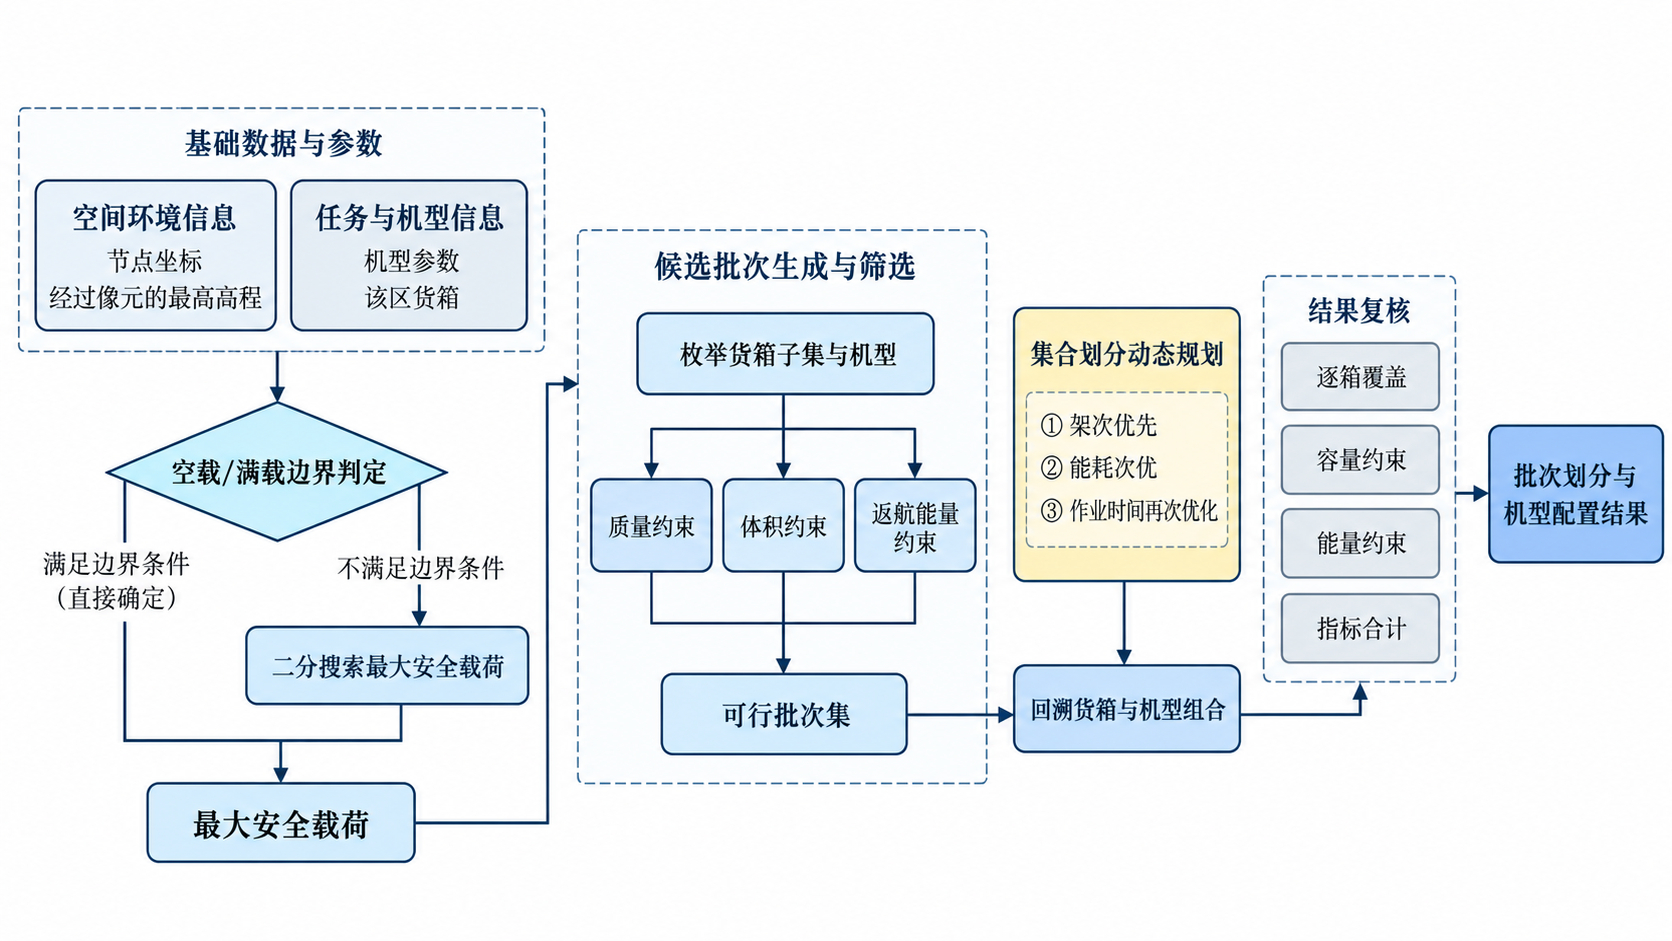
\includegraphics[width=\textwidth]{figures/q1/figure5.png}
\caption{单点运输能力与货箱组批求解流程}\label{fig:q1-flow}
\end{figure}

\subsection{安全载荷计算结果}
按修正后的DEM穿越像元口径，对15个服务区和3种机型共45个组合重新计算最大安全载荷，结果如图~\ref{fig:q1-safe-payload}所示。45个组合均可完成空载返航，其中A型在全部服务区均达到25~kg额定载荷；B型仅在S008受能量约束，最大安全载荷为28.632~kg；C型在S002、S003、S004、S008和S012分别降至68.554、68.235、63.259、58.436和68.015~kg，其余服务区均达到80~kg额定载荷。S008--C的载荷保持率最低，为73.0\%。该图只呈现安全载荷的空间差异，差异由航程、沿途最高地形与机型载荷航程参数共同进入式~\eqref{eq:safe-payload}后产生。

\begin{figure}[H]
  \centering
  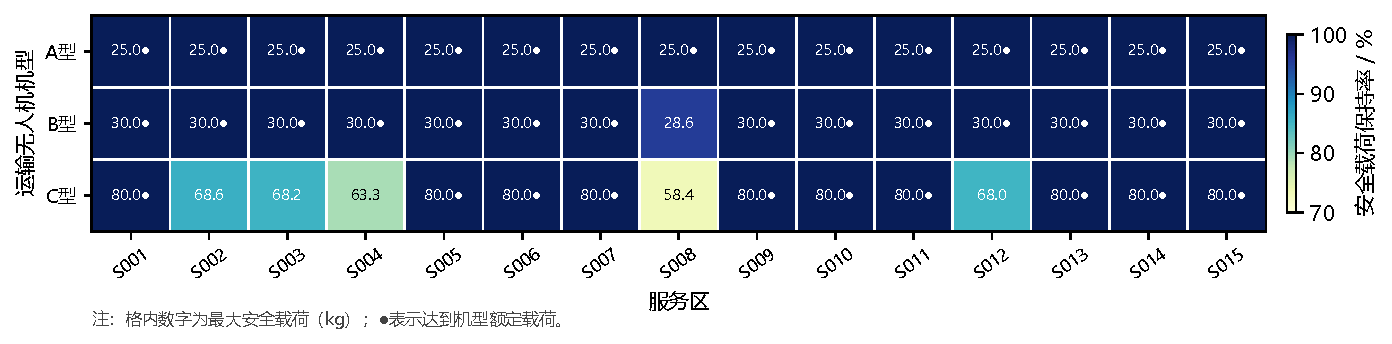
\includegraphics[width=\textwidth]{figures/q1/q1_safe_payload_heatmap.pdf}
  \caption{不同服务区与运输无人机机型的最大安全载荷}
  \label{fig:q1-safe-payload}
\end{figure}

\subsection{组批方案与结果分析}
将各服务区货箱分别代入集合划分动态规划后，80个货箱均被覆盖且恰好出现一次，不存在遗漏、重复或跨区组批。最终得到18个单点往返架次，其中B型与C型各承担9架次，A型未被选用；S001、S002和S003各需要2架次，其余12个服务区各需要1架次。全部架次的累计往返能耗为59.240~kWh，累计作业时间为9.111~h。这里的累计时间是各独立架次作业时长之和，不代表考虑实体机和共享电池后的调度完工时间，后者在问题二中计算。

\begin{table}[htbp]
  \centering
  \caption{问题一组批结果汇总}
  \label{tab:q1-summary}
  \begin{tabular}{lr}
    \toprule
    指标 & 计算结果 \\
    \midrule
    唯一覆盖货箱数 & 80箱 \\
    总架次数 & 18架次 \\
    A/B/C型架次数 & 0/9/9 \\
    累计往返能耗 & 59.240~kWh \\
    累计作业时间 & 9.111~h \\
    \bottomrule
  \end{tabular}
\end{table}

为判断各批次由哪类容量约束主导，定义质量、体积和安全可用能量利用率分别为
\begin{equation}
\eta_r^m=\frac{w_r}{Q_{g_r}},\qquad
\eta_r^v=\frac{v_r}{V_{g_r}},\qquad
\eta_r^e=\frac{E_r}{(1-\rho_{g_r})E_{g_r}^{use}}.
\end{equation}
图~\ref{fig:q1-utilization}给出18个批次的三类利用率。质量、体积和能量利用率的均值分别为78.7\%、77.2\%和68.4\%。若以三项利用率中的最大者作为该批次最紧约束，则9个批次最接近体积上限、5个最接近质量上限、4个最接近能量上限。Q1--S001--02的质量与体积利用率最高，分别为97.5\%和94.0\%；Q1--S004--01的能量利用率最高，达到96.5\%。这说明未达到额定载质量并不等于装载低效：完整货箱不可拆分，且部分批次会先触及舱容或安全能量边界。

\begin{figure}[H]
  \centering
  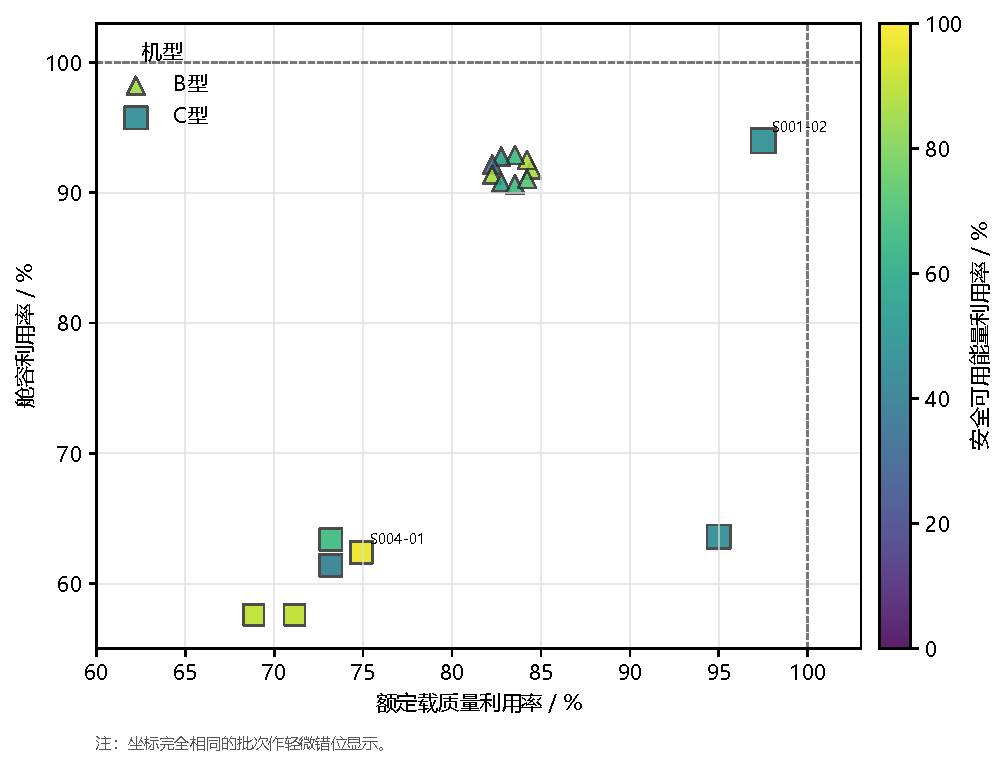
\includegraphics[width=0.82\textwidth]{figures/q1/q1_batch_utilization.pdf}
  \caption{问题一最终运输批次的质量、体积与能量利用率}
  \label{fig:q1-utilization}
\end{figure}
